%!TEX root = main.tex

\section{Motivation}

\begin{frame}{Motivation}{Password Hashing Function?}
	\center \Large
	Can't we just store passwords in plain?\visible<2->{\footnote<2->{\tiny \url{blog.ebay.com/ebay-inc-ask-ebay-users-change-passwords}}\footnote<2->{\tiny \url{blogs.adobe.com/conversations/2013/10/important-customer-security-announcement.html}}}
	\visible<2->{
	\begin{columns}[T]
		\begin{column}{.45\textwidth}
			\vspace{1cm}
			
\includegraphics[width=\textwidth]{data/wikimedia/logo_ebay.png}
		\end{column}
		\begin{column}{.45\textwidth}
			
\includegraphics[width=\textwidth]{data/wikimedia/logo_adobe.png}
		\end{column}
	\end{columns}
	}
\end{frame}

\begin{frame}{Motivation}{Secure Storage?}
	\center
	\begin{tikzpicture}[node distance=4cm]
		\node (start) [startstop] {Password};
		\node (salt) [startstop, below of=start, node distance=2cm, opacity=0] {Salt};
		\node (hash) [process, right of=start] {Hash};
		\node (hashfkt) [plainnode, above of=hash, node distance=2cm, visible on=<-1>] {MD5 \\ SHA\{1,~2,~3\} \\ \ldots};
		\node (hashfkt) [plainnode, above of=hash, node distance=2cm, visible on=<2->, cross out, draw=red] {MD5 \\ SHA\{1,~2,~3\} \\ \ldots};
		\node (stop) [right of=hash] {
\includegraphics[width=1cm]{data/fingerprint.pdf}};

		\draw [arrow] (start) -- (hash);
		\draw [arrow] (hash) -- (stop);
		\draw [arrow] (hashfkt) -- (hash);
	\end{tikzpicture}

	\visible<2->{\textbf{don't use standard hash functions}}
\end{frame}

\begin{frame}{Motivation}{Secure Storage!}
	\center
	\begin{tikzpicture}[node distance=4cm]
		\node (start) [startstop] {Password};
		\node (cost) [startstop, above of=start, node distance=2cm] {Cost};
		\node (salt) [startstop, below of=start, node distance=2cm] {Salt};
		\node (hash) [process, right of=start] {Hash};
		\node (hashfkt) [plainnode, above of=hash, node distance=2cm] {PBKDF2 \\ \textbf{bcrypt} \\ scrypt};
		\node (stop) [right of=hash] {
\includegraphics[width=1cm]{data/fingerprint.pdf}};

		\draw [arrow] (start) -- (hash);
		\draw [arrow] (cost) -- (hashfkt);
		\draw [arrow] (salt) -| (hash);
		\draw [arrow] (hash) -- (stop);
		\draw [arrow] (hashfkt) -- (hash);
	\end{tikzpicture}
	\\[5.5mm]
\end{frame}

\begin{frame}{Motivation}
	\begin{block}{Why do we care?}
		\begin{itemize}
			\item password cracking has an inherent parallel structure
			\item FPGAs enable to exploit this parallelism
		\end{itemize}
		\begin{itemize}
			\item bcrypt claims to resist hardware optimizations
			\item currently available implementations\footnote{K.~Malvoni et~al.
				Are Your Passwords Safe: Energy-Efficient Bcrypt Cracking with
				Low-Cost Parallel Hardware {\em 8th USENIX Workshop on Offensive
				Technologies (WOOT 14), 2014}}
				suffer from interface bottlenecks and instable operations
		\end{itemize}
	\end{block}
\end{frame}

\section{bcrypt}

\begin{frame}{What is bcrypt?}
	Introduced in 1999 by Provos and Mazi\`{e}res.\footnote{\tiny \url{www.usenix.org/events/usenix99/full_papers/provos/provos.pdf}}
	Implemented in OpenBSD 2.1, Ruby on Rails, and PHP as standard password hash.

	\begin{columns}[T]
		\begin{column}{.47\textwidth}
			\begin{block}{bcrypt}
				\begin{itemize}
					\item cost-parameterized
					\item based on modified Blowfish
				\end{itemize}
			\end{block}
		\end{column}
		\visible<2->{
		\begin{column}{.47\textwidth}
			\begin{block}{Blowfish}
				\begin{itemize}
					\item symmetric blockcipher
					\item Feistel network
				\end{itemize}
			\end{block}
		\end{column}}
	\end{columns}
\end{frame}

\begin{frame}{bcrypt}
	\begin{columns}[T]
		\begin{column}{.47\textwidth}
			\begin{block}{Structure}
				\begin{itemize}
					\item setup state, using the \emph{password} and \emph{salt} as key with
						 modified Blowfish key schedule
					\item encrypt magic value
					\item output ciphertext as hash
				\end{itemize}
			\end{block}
		\end{column}
		\visible<2->{
		\begin{column}{.47\textwidth}
			\begin{block}{Work}
				\begin{itemize}
					\item needs $(2^{\text{cost}+1}+1) \cdot 521$ Blowfish encryptions\\(roughly $2^{\text{cost}+10}$)
					\item[]
					\item needs $3 \cdot 64$ Blowfish encryptions
				\end{itemize}
			\end{block}
		\end{column}}
	\end{columns}
\end{frame}

\section{Design of Implementation}

\begin{frame}{Implementation}{Cracker}
		\center 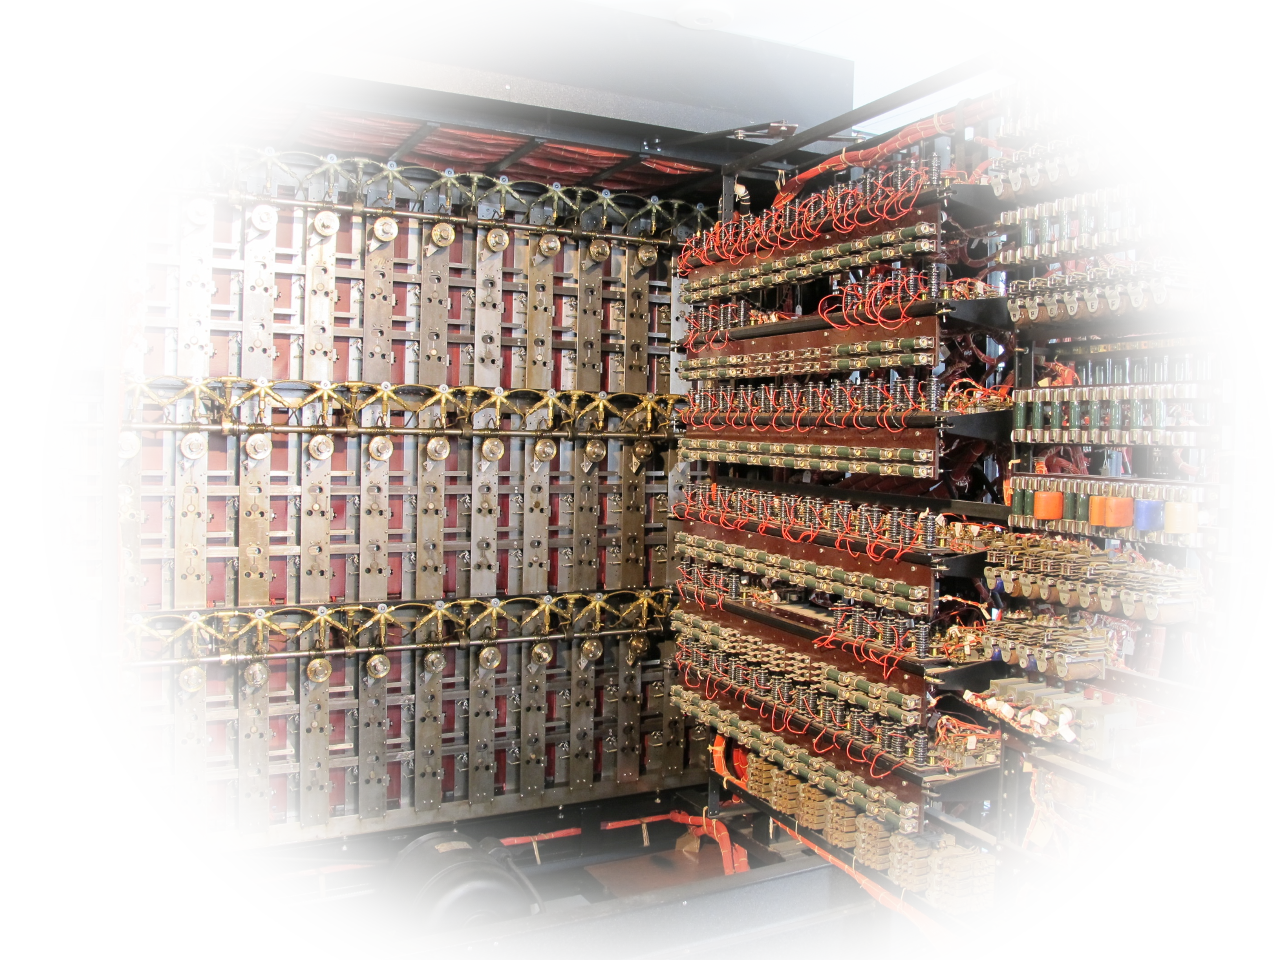
\includegraphics[height=70mm]{data/flickr/bombe_bletchly_park.png}
\end{frame}

\begin{frame}{Target Platforms}
	\begin{columns}[T]
		\begin{column}{.45\textwidth}
			Low cost, low power FPGA
			\begin{block}{Zedboard}
				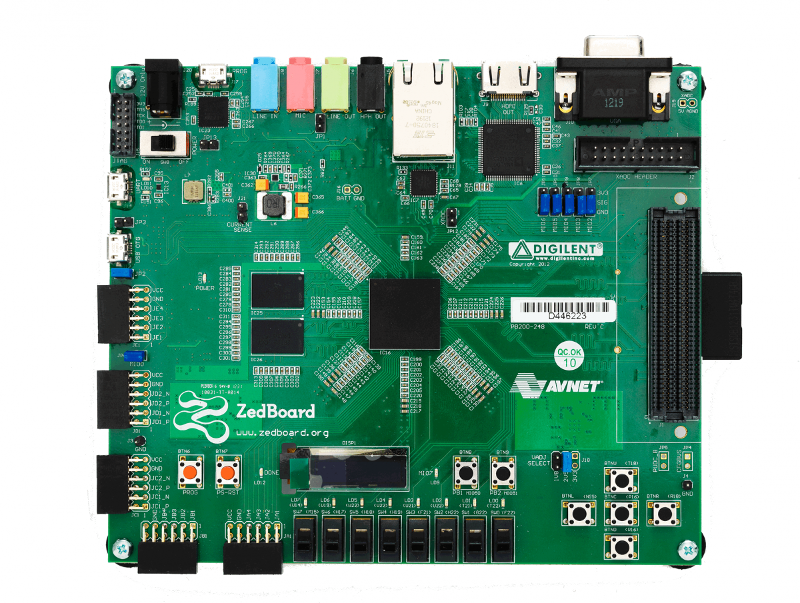
\includegraphics[width=\textwidth]{data/zedboard.png}
			\end{block}
		\end{column}
		\begin{column}{.45\textwidth}
			\visible<2->{
			High Performance FPGA
			\begin{block}{Virtex-7}
				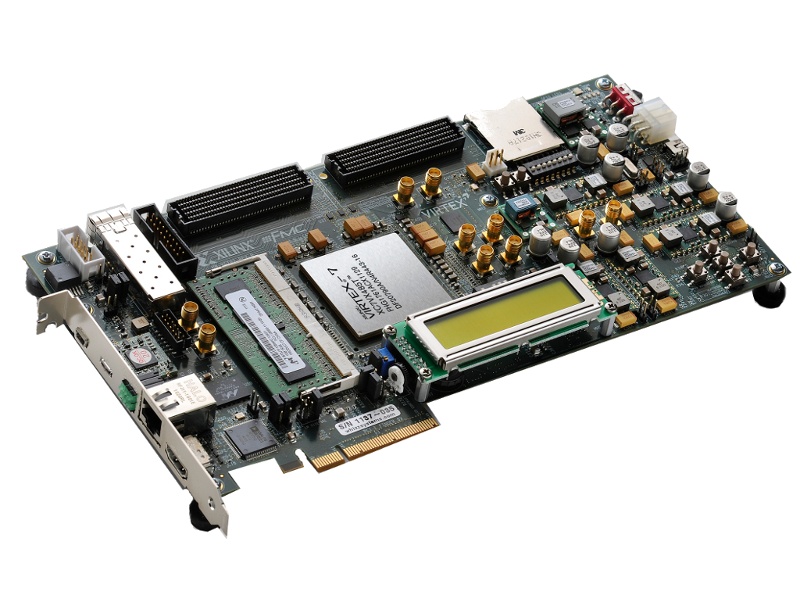
\includegraphics[width=\textwidth]{data/virtex7.png}
			\end{block}
			}
		\end{column}
	\end{columns}
\end{frame}
% Virtex-7 ~ 13 times larger than zedboard

\begin{frame}{Optimization}
	\center \Huge
	Optimization Goal?
\end{frame}

\begin{frame}{Optimization}
	\center \Huge
	Low Area Footprint (bcrypt)

	\visible<2->{High-Speed (Blowfish)}
\end{frame}

%\begin{frame}{Design}
%	\begin{block}{API}
%		\begin{itemize}
%			\item keep API minimalistic $\Rightarrow$ low bandwidth interface
%			\item transfer target \emph{salt} and \emph{hash}, start cracker
%			\item on success, read \emph{password}
%		\end{itemize}
%	\end{block}
%	\begin{block}{Password Generation}
%		\begin{itemize}
%			\item on-chip password generation
%			\item no bandwidth
%			\item split password range at synthesis-time
%		\end{itemize}
%		\begin{itemize}
%			\item alternatively replace generator with interface for dictionary attacks
%		\end{itemize}
%	\end{block}
%\end{frame}

\begin{frame}{Design}
	\begin{block}{First Attempt}
		\center
		\only<-1>{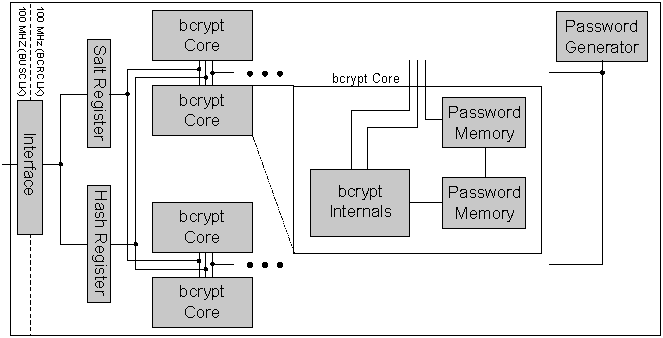
\includegraphics[width=.90\textwidth]{data/bcrypt_design_first_attempt.pdf}}
		\only<2->{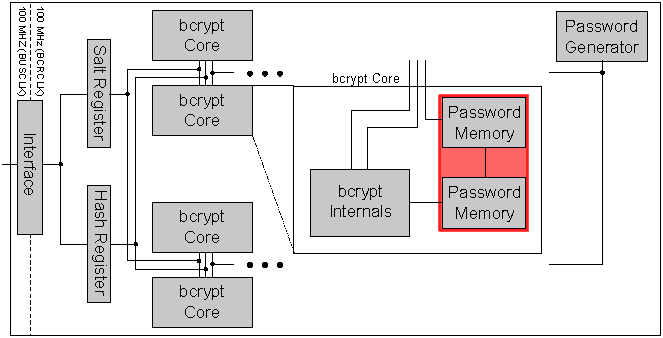
\includegraphics[width=.90\textwidth]{data/bcrypt_design_first_attempt_red.pdf}}
	\end{block}
\end{frame}

%\begin{frame}{Design}
%	\begin{block}{bcrypt Core}
%		\begin{itemize}
%			\item memory for SBoxes, subkeys, key and initial values
%			\item estimated almost no logic needed for algorithm\\consists mainly of BRAM access
%		\end{itemize}
%	\end{block}
%	\begin{alertblock}{Problematic}
%		\begin{itemize}
%			\item memory for password storage\\registers require too much logic
%			\item one core consumes more LUTs than expected\\need to optimize FSM, share resources
%		\end{itemize}
%	\end{alertblock}
%\end{frame}

\begin{frame}{Design}
	\begin{block}{Quad Core}
		\center 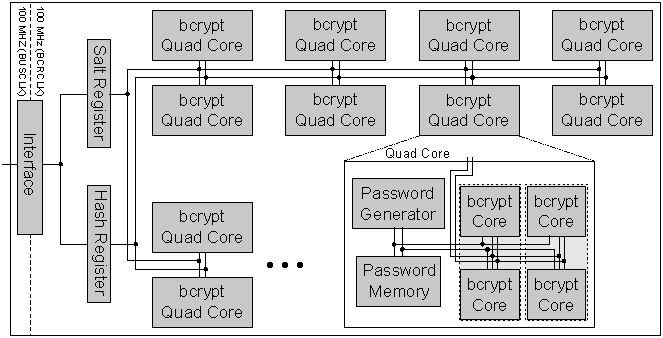
\includegraphics[width=.90\textwidth]{data/bcrypt_design_overview.pdf}
	\end{block}
\end{frame}

%\begin{frame}{Design}
%	\begin{block}{Quad Core}
%		\begin{itemize}
%			\item bundle four bcrypt cores together
%			\item store four passwords in one BRAM
%			\item during initialization, password generator can access BRAM
%			\item core0, core1 and core2, core3 access the BRAM alternately
%		\end{itemize}
%	\end{block}
%	\begin{exampleblock}{Advantages}
%		\begin{itemize}
%			\item cores need access only during begin of \texttt{ExpandKey}\\thus,
%						they only diverge by 36 clock cycles
%			\item saves more than 4000 LUTs per quad core\\
%						\SI{20}{\percent} per single core
%		\end{itemize}
%	\end{exampleblock}
%\end{frame}

%\begin{frame}{Design}
%	\begin{block}{Password Generator}
%		\center 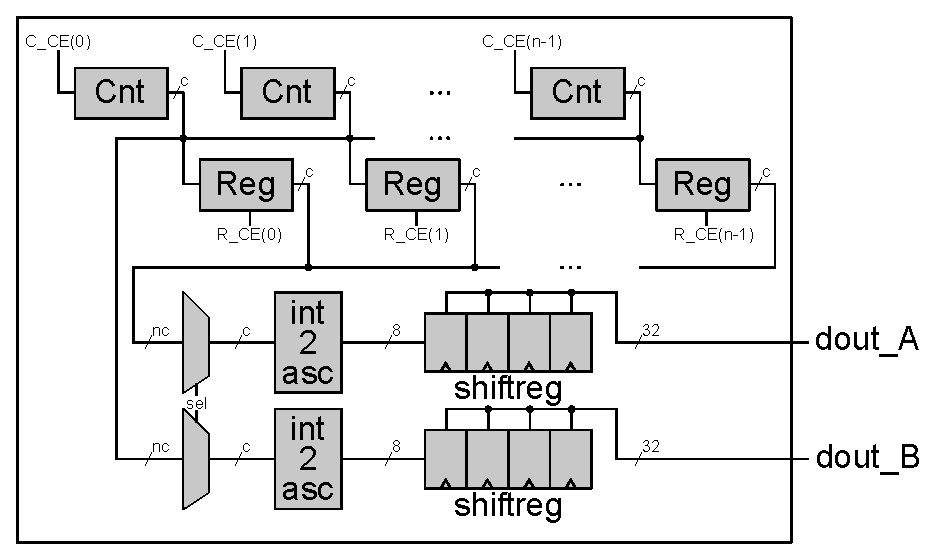
\includegraphics[width=.90\textwidth]{data/password_gen.pdf}
%	\end{block}
%\end{frame}

\begin{frame}{Design}{Blowfish Core}
	\begin{columns}[T]
		\begin{column}{.45\textwidth}
			\begin{block}{One Round}
				\center 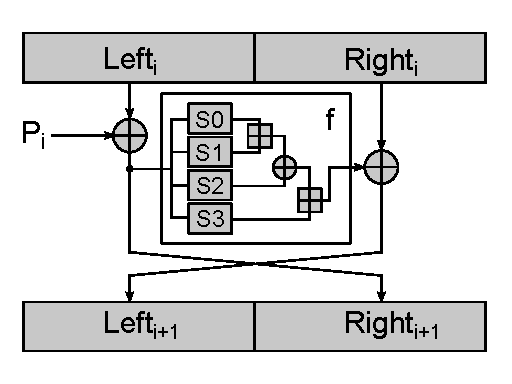
\includegraphics[width=.90\textwidth]{data/blowfish_feistel.pdf}
			\end{block}
		\end{column}
		\visible<2->{
			\begin{column}{.45\textwidth}
				\begin{alertblock}{Problematic}
					\begin{itemize}
						\item SBox addresses can not be computed in the same clock as the look up is used
						\item needs 2 clock cycles per round
					\end{itemize}
				\end{alertblock}
			\end{column}
		}
	\end{columns}
\end{frame}

\begin{frame}{Design}{Blowfish Core Retimed}
	\begin{columns}[T]
		\begin{column}{.45\textwidth}
			\begin{block}{Prefetch}
				\center 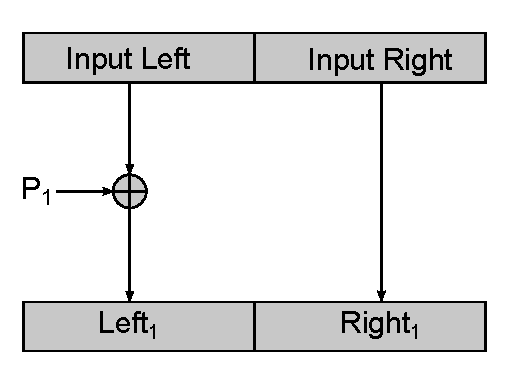
\includegraphics[width=.90\textwidth]{data/blowfish_prefetch.pdf}
			\end{block}
		\end{column}
		\begin{column}{.45\textwidth}
			\begin{block}{Retimed Round}
				\center 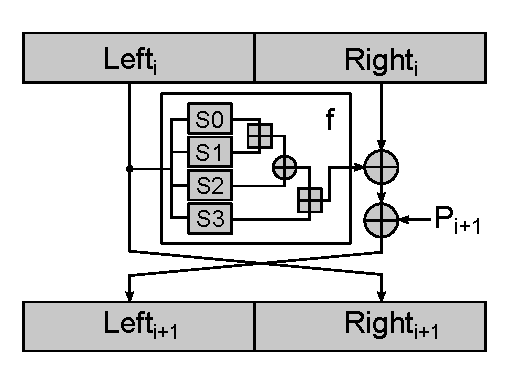
\includegraphics[width=.90\textwidth]{data/blowfish_retimed.pdf}
			\end{block}
		\end{column}
	\end{columns}

	\begin{columns}[T]
		\begin{column}{.975\textwidth}
			\begin{exampleblock}{Advantages}
				\begin{itemize}
					\item needs only 1 clock per round
				\end{itemize}
			\end{exampleblock}
		\end{column}
	\end{columns}
\end{frame}

\section{Results}

\begin{frame}{Resulting Resources}
	\begin{block}{Zedboard}
		\begin{itemize}
			\item estimations for one zedboard:
			\item[] 40 cores as upper bound, BRAMs as limiting resource
			\item first design attempt (password in registers):
			\item[] 12 cores fit, LUT utilization way to high
			\item Quad Core Design:
			\item[] 40 cores fit, while using \enquote{big} interface
		\end{itemize}
	\end{block}
	\begin{block}{Virtex-7}
		\begin{itemize}
			\item Quad Core Design:
			\item[] 316 cores per FPGA
		\end{itemize}
	\end{block}
\end{frame}

\begin{frame}{Resulting Resources}
	\begin{block}{Resource utilization of design and submodules}
		\begin{table}[tp]
			\centering
			\begin{tabular}{l r r r r}
				\toprule
								   &   LUT   &   FF    &  Slice  &  BRAM   \\
				\midrule
				Overall            &  64.8\% & 13.06\% & 93.29\% & 95.71\% \\
				\midrule
				Quad Core          &  2,777  &    720  &    801  &   13    \\
				Single Core        &    617  &    132  &    197  &    3    \\
				Blowfish Core      &    354  &     64  &     71  &    0    \\
				Password Generator &    216  &    205  &     81  &    0    \\
				\bottomrule\\
			\end{tabular}
		\end{table}
	\end{block}
\end{frame}

\begin{frame}{Resulting Hashrates}
	\begin{block}{Compared to}
		\begin{table}[tp]
			\centering
			\begin{tabular}{l c c c c}
				\toprule
					& \multicolumn{2}{c}{cost factor 5} & \multicolumn{2}{c}{cost factor 12} \\
					& $\frac{\text{Hashes}}{\text{Second}}$
					& $\frac{\text{Hashes}}{\text{Watt Second}}$
					& $\frac{\text{Hashes}}{\text{Second}}$
					& $\frac{\text{Hashes}}{\text{Watt Second}}$
					\\
				\midrule
				{\bf Zedboard}  & {\bf 6,511} & {\bf 1,550} & {\bf 51.95} & {\bf 12.37} \\
				Malvoni~(GSoC)  &        780  &             &             &             \\
				Malvoni~et~al.  &      4,571  &      682.24 &      64.83  &       9.68  \\
				\midrule
				Virtex-7        &     51,437  &      2,572  &     410.4   &      20.52  \\
				\midrule
				Xeon E3-1240    &      6,210  &       20.7  &      50     &       0.17  \\
				GTX 750 Ti      &      1,920  &        6.4  &      15     &       0.05  \\
				\bottomrule
			\end{tabular}
		\end{table}
	\end{block}
\end{frame}

\begin{frame}{Brute Force Attack}
	\begin{block}{Cost 5}
		%!TEX root = main.tex

\begin{figure} \centering
	\begin{tikzpicture}
	\pgfplotsset{
		height=.5\textheight, width=.8\textwidth,
		scale only axis,
		legend columns=2,
		legend style={at={(0.5,0.75)},
					  xshift=0.25cm,
					  yshift=1.5cm,
					  anchor=north west,
					  nodes=right,
					  font=\scriptsize,
					 },
		every axis plot post/.append style={
			mark=none,
			domain=0:50,
			samples=100,
			thick},
		}
	\begin{axis}[
		scatter/classes={a={mark=|,black}},
		axis y line=left,
		axis x line=bottom,
		x tick label style={font=\scriptsize},
		y tick label style={font=\scriptsize},
		xlabel style={font=\footnotesize},
		xlabel=Number of attacked passwords,
		ylabel style={font=\footnotesize},
		ylabel=Total costs in \$1\,000\,000,
		%xtick={25, 50, 75, 100, 125, 150, 175},
		xmin=1, xmax=50,
		ytick={5000000, 7000000, 10000000, 15000000, 20000000},
		yticklabels={$5$, $7$, $10$, $15$, $20$},
		ymin=4000000, ymax=25000000,
		ymode=log,
		cycle list name=linestyles*
		]
		\addplot+[color=black,only marks,scatter,scatter src=explicit symbolic] coordinates{
			(2.75, 10525390.42) [a]
			(1.91, 5895676.33) [a]
			(20.33, 11335789.16) [a]
			(1.43, 5752687.56) [a]
			(24.86, 11544263.66) [a]
			(8.69, 7897759.68) [a]
			(1017.0, 8177871.0) [a]
		};
		\addplot+[color=blue]{5330652+295327*x}; %CPU
		\addplot+[color=brown]{7896960+955217*x}; %GPU
		\addplot+[color=orange]{5936853+225588*x}; %CPU+GPU
		\addplot+[color=green]{5749275+2388*x}; %Virtex7
		\addplot+[color=red]{4146681+3963*x}; %zedboard
		\addplot+[color=purple]{5878532+8961*x}; %OWzb
		\legend{
			break-even, CPU$^*$, GPU$^*$, CPU+GPU$^*$,
			Virtex-7, zedboard, Malvoni~et~al.
			}
	\end{axis}
	\end{tikzpicture}
\end{figure}

	\end{block}
\end{frame}

%\begin{frame}{Dictonary Attack}
%	\begin{block}{Cost 12}
%		\input{plot_dict.tex}
%	\end{block}
%\end{frame}

%\begin{frame}{Optimizations}
%	\begin{block}{Future Work}
%		\begin{itemize}
%			\item interleaved design
%			\item usage of password generator
%			\item mangling rules
%		\end{itemize}
%	\end{block}
%\end{frame}
